\documentclass[letterpaper,journal]{IEEEtran}
\usepackage{amsmath,amssymb,bm}
\usepackage{cite}
\usepackage{graphicx}
\graphicspath{{figure/}}
\usepackage{tikz}
\usetikzlibrary{positioning,calc}
\usepackage{url,hyperref}
\hypersetup{hidelinks}
\newtheorem{lemma}{Lemma}
\hyphenation{op-tical net-works semi-conduc-tor IEEE-Xplore}

\begin{document}

\title{Fake-Peak Artificial Noise for Sensing-Location Privacy in Cell-Free Massive MIMO ISAC}

% The paper headers
\markboth{IEEE Transactions on Vehicular Technology,~Vol.~XX, No.~XX, XXXX~XXXX}%
{Xu \MakeLowercase{\textit{et al.}}: Fake-Peak Artificial Noise for Sensing-Location Privacy in Cell-Free Massive MIMO ISAC}

\maketitle

\begin{abstract}
Multi-static cell-free massive MIMO integrated sensing and communication is vulnerable to internal sensing leakage, since a served user can reconstruct transmit beampatterns and fuse their dominant directions to infer a target location. Conventional artificial noise (AN) under strict per-access-point (AP) physical-channel nulling is absent from the raw observations used by this internal adversary. We instead exploit the receive-processing asymmetry between legitimate post-combining detection and raw-sample reconstruction. Network-wide effective-channel nulling cancels the AN at the combiner outputs while preserving it in the adversary's multi-antenna observations. Within the resulting null space, the AN is shaped to generate AP-dependent dominant directions consistent with a common virtual location. A joint beam design maximizes the sensing signal-to-noise ratio under communication quality and per-AP power constraints. Simulations show that, at an AN-power ratio of approximately $0.50$, the proposed design lowers the target-localization success rate from $35.8\%$ without AN to $2.8\%$, with a $3.6$~dB sensing-SNR loss.

% At $-10$~dB channel-estimation NMSE, the error-averaged design reduces communication outage from $18.6\%$ to $1.6\%$ under the adopted LMMSE error model.
\end{abstract}

\begin{IEEEkeywords}
Cell-free massive MIMO, integrated sensing and communication, sensing privacy, artificial noise, internal adversary.
\end{IEEEkeywords}

\section{Introduction}
Integrated sensing and communication (ISAC) is a key technology for sixth-generation networks, enabling data transmission and environmental sensing through shared spectrum and hardware \cite{liu2022jsac}. Cell-free massive MIMO (CF-mMIMO) is especially suitable for ISAC, since geographically distributed access points (APs) coordinated by a central processor form a virtual array that jointly illuminates targets \cite{demirhan2024cellfreetcom,behdad2024multistatic}. The same distributed configuration, however, enlarges the attack surface for sensing-information leakage.

Physical-layer security has long been used to protect confidential messages against eavesdropping. In the seminal artificial-noise (AN) design of Goel and Negi \cite{goel2008guaranteeing}, noise is radiated in the null space of the legitimate channel, so that the eavesdropper is degraded while the intended user is unaffected. These ideas have been extended to secure ISAC, where the illuminated target is treated as an information eavesdropper and the precoding and AN covariance are optimized to degrade its channel \cite{su2021secure,rivetti2024secure,ren2023securecf}. A complementary line of work protects the sensing function itself. Low-probability-of-intercept power allocation has been studied for integrated multi-static radar and communication systems \cite{shi2020lpi}, and the target-location distribution has been exploited as prior knowledge in secure ISAC beamforming \cite{hou2024targetdist}. Notably, Zou \emph{et al.} \cite{zou2024securing} model a served communication user as a sensing eavesdropper and design AN-aided beamforming to limit its sensing mutual information, while Han \emph{et al.} \cite{han2026sensingsecure} shape the ISAC ambiguity function to create ghost targets in an unauthorized receiver's range profile.

This correspondence addresses the internal threat identified in \cite{dasilva2023multistaticcf}, where a served user reconstructs the transmit beampattern of each AP and then fuses the AP-dependent directions to localize the target. We refer to this as the \emph{reconstruction attack}. Such an adversary is difficult to defend against because it is indistinguishable from an ordinary user at the protocol level. In particular, classical AN designs suppress the AN on the legitimate users' channels so that intended reception is unaffected \cite{goel2008guaranteeing,rivetti2024secure}. However, when the adversary is itself a served user, such nulling also removes the AN from its own received samples and therefore provides no protection.

The contributions of our study are twofold. First, we find that data detection operates on post-combining scalar observations, whereas the reconstruction attack exploits raw samples before combining. Exploiting this receive-processing asymmetry, we null the AN on the network-wide effective channels rather than on the physical channels, thereby retaining the AN in the adversary's raw observations. Second, within this subspace we design a fake-peak AN beam whose AP-dependent deceptive directions are generated from a common virtual location, and jointly optimize the communication, sensing, and AN beams by an alternating concave-convex procedure (CCCP)--minimum mean square error (MMSE) algorithm under quality-of-service (QoS) and per-AP power constraints.

% Simulations show that the target-localization success rate drops from $35.8\%$ to $2.8\%$ at a moderate AN-power ratio ($\eta\approx0.50$), subject to the prescribed communication constraints and a moderate sensing-SNR loss.

\emph{Notation:} Boldface upper- and lower-case letters denote matrices and vectors, and $\mathbb{C}$ is the complex field. $(\cdot)^*$, $(\cdot)^H$, $(\cdot)^T$, $(\cdot)^\dagger$, $\mathrm{Tr}(\cdot)$, $\|\cdot\|$, and $\|\cdot\|_F$ are the conjugate, conjugate transpose, transpose, pseudoinverse, trace, Euclidean norm, and Frobenius norm. $\mathbf{I}_N$ is the $N\times N$ identity matrix, $\mathcal{N}(\cdot)$ the null space, $\Re\{\cdot\}$ the real part, $\angle(\cdot)$ the phase angle, $\mathbb{E}\{\cdot\}$ the expectation, $\Pr\{\cdot\}$ the probability, and $\jmath=\sqrt{-1}$. $\mathbf{A}\succ\mathbf{0}$ and $\mathbf{A}\succeq\mathbf{0}$ mean positive definite and positive semidefinite, and $\mathcal{CN}(\mathbf{0},\mathbf{R})$ denotes a circularly symmetric complex Gaussian distribution.

\section{System and Threat Model}
\label{sec:model}

We consider a CF-mMIMO ISAC network with $N_{\mathrm{tx}}$ transmit APs, $N_{\mathrm{rx}}$ receive APs, and $N_{\mathrm{UE}}$ multi-antenna users. Each transmit AP employs an $M_{\mathrm{tx}}$-element uniform linear array with half-wavelength spacing, and each user has $M_{\mathrm{UE}}$ antennas. The APs are coordinated by a central processor to serve the users and illuminate a point target. Accordingly, the signal emitted by AP $k$ at time index $n$ can be expressed as
\begin{equation}
\mathbf{x}_k[n]=\sum_{i=1}^{N_{\mathrm{UE}}}\mathbf{w}_{i,k}s_i[n]+\mathbf{w}_{t,k}s_t[n],
\label{eq:xk}
\end{equation}
where $\mathbf{w}_{i,k}\in\mathbb{C}^{M_{\mathrm{tx}}\times 1}$ is the beam for user $i$, $\mathbf{w}_{t,k}\in\mathbb{C}^{M_{\mathrm{tx}}\times 1}$ is the sensing beam, and the symbols $\{s_i[n]\}_{i=1}^{N_{\mathrm{UE}}}$ and $s_t[n]$ are mutually independent with zero mean and unit variance. The AP--user channel is modeled as $\mathbf{H}_{i,k}=\sqrt{\beta_{i,k}}\,\mathbf{G}_{i,k}\in\mathbb{C}^{M_{\mathrm{UE}}\times M_{\mathrm{tx}}}$, where $\mathbf{G}_{i,k}$ has i.i.d. $\mathcal{CN}(0,1)$ entries and $\beta_{i,k}$ denotes the large-scale fading coefficient. The system operates in time-division duplex mode. Exploiting channel reciprocity, each transmit AP estimates $\mathbf{H}_{i,k}$ from $\tau_{\mathrm{p}}$-length orthogonal uplink pilots of per-antenna power $p_i^{\mathrm{p}}=P_{\mathrm{p}}/M_{\mathrm{UE}}$, where $P_{\mathrm{p}}$ is the total pilot power per user, received with i.i.d. $\mathcal{CN}(0,\sigma_{\mathrm{p}}^2)$ noise. This yields the linear minimum mean square error (LMMSE) estimate $\widehat{\mathbf{H}}_{i,k}$ used for beam design.

In the downlink transmission, the received signal at user $i$ and time index $n$ is $\mathbf{y}_i[n]=\sum_k\mathbf{H}_{i,k}\mathbf{x}_k[n]+\mathbf{n}_i[n]$, where $\mathbf{n}_i[n]\sim\mathcal{CN}(\mathbf{0},\sigma_i^2\mathbf{I}_{M_{\mathrm{UE}}})$ denotes the noise, and user $i$ applies a combiner $\mathbf{u}_i\in\mathbb{C}^{M_{\mathrm{UE}}\times 1}$. For multi-static sensing, AP $k$ illuminates the target at angle $\phi_k$ with steering vector $\mathbf{a}(\phi)=[1,e^{\jmath\pi\sin\phi},\ldots,e^{\jmath\pi(M_{\mathrm{tx}}-1)\sin\phi}]^T$. With $\mathbf{W}_k\triangleq[\mathbf{w}_{1,k},\ldots,\mathbf{w}_{N_{\mathrm{UE}},k},\mathbf{w}_{t,k}]$, the average sensing SNR is
\begin{equation}
\gamma_t=\sum_{k=1}^{N_{\mathrm{tx}}}c_k\left\|\mathbf{a}^H(\phi_k)\mathbf{W}_k\right\|_F^2,\quad c_k=\frac{\sum_{r=1}^{N_{\mathrm{rx}}}\xi_{r,k}^2 g_{r,k}}{N_{\mathrm{rx}}\sigma_{\mathrm{rx}}^2},
\label{eq:snr-sensing}
\end{equation}
where $g_{r,k}=\lambda_c^2/[(4\pi)^3d_{t,k}^2d_{t,r}^2]$ is the two-way path gain, in which $\lambda_c$ is the carrier wavelength and $d_{t,k}$ and $d_{t,r}$ denote the transmit-AP-$k$--target and target--receive-AP-$r$ distances, $\xi_{r,k}^2$ is the scattering power absorbing the target radar cross section and the receive array gain, and $\sigma_{\mathrm{rx}}^2$ is the receive noise power.

One served user, indexed by $a$, is treated as an internal adversary. It knows its own pilots, data symbols, combiner $\mathbf{u}_a$, and the transmit-AP positions, and can form its own estimate $\widehat{\mathbf{H}}_{a,k}^{\mathrm{adv}}$ of its channel $\mathbf{H}_{a,k}$. Following \cite{dasilva2023multistaticcf}, it is assumed to separate its received samples into per-AP components. The attack must operate on the raw multi-antenna samples, since applying $\mathbf{u}_a$ would collapse each snapshot into a scalar and leave the $M_{\mathrm{tx}}$-dimensional transmit-vector recovery underdetermined. After decoding its own data symbol $s_a[n]$, the adversary subtracts its data component using its channel estimate $\widehat{\mathbf{H}}_{a,k}^{\mathrm{adv}}$, which leaves $\widetilde{\mathbf{y}}_{a,k}[n]=\widehat{\mathbf{H}}_{a,k}^{\mathrm{adv}}\widetilde{\mathbf{x}}_k[n]+\widetilde{\mathbf{n}}_{a,k}^{\mathrm{adv}}[n]$ with the non-self transmit component $\widetilde{\mathbf{x}}_k[n]=\sum_{j\neq a}\mathbf{w}_{j,k}s_j[n]+\mathbf{w}_{t,k}s_t[n]$, and $\widetilde{\mathbf{n}}_{a,k}^{\mathrm{adv}}[n]$ collecting the receiver noise and the residual caused by adversary-side channel-estimation errors. It then applies an expectation-maximization routine to obtain $\widehat{\mathbf{x}}_k[n]\approx\widetilde{\mathbf{x}}_k[n]$, and forms the AP-dependent beampattern from the sample covariance over the available snapshots, i.e.,
\begin{equation}
\widehat{B}_k(\theta)=\mathbf{a}^H(\theta)\mathbf{R}_{\widehat{\mathbf{x}}_k}\mathbf{a}(\theta),\quad \mathbf{R}_{\widehat{\mathbf{x}}_k}=\frac{1}{N}\sum_{n=1}^{N}\widehat{\mathbf{x}}_k[n]\widehat{\mathbf{x}}_k^H[n],
\label{eq:beampattern}
\end{equation}
where $\theta$ denotes the search angle scanned by the adversary and $N$ is the number of available snapshots. The target position is then estimated by fusing the direction lines emanating from each AP along the dominant angle of $\widehat{B}_k(\theta)$, taking the cell of a search grid of resolution $\Delta_{\mathrm{g}}$.

\section{Channel-Nulling-Based Fake-Peak AN Design}
\label{sec:design}
\label{sec:nulling}
% This section formalizes receive-processing asymmetric nulling. We distinguish the legitimate post-combining operator from the raw-observation operator, compare physical- and effective-channel nulling, and adopt network-wide effective-channel nulling under the coherent CF-mMIMO model.

\subsection{Receive-Processing Asymmetric Nulling}
\label{subsec:asym}
\label{subsec:hierarchy}

We augment the transmit signal at AP $k$ as
\begin{equation}
\mathbf{x}_k[n]=\sum_{i=1}^{N_{\mathrm{UE}}}\mathbf{w}_{i,k}s_i[n]+\mathbf{w}_{t,k}s_t[n]+\mathbf{z}_ks_z[n],
\label{eq:xk-an}
\end{equation}
where $\mathbf{z}_k\in\mathbb{C}^{M_{\mathrm{tx}}\times 1}$ is the AN beam, and $s_z[n]$ is a common AN symbol with zero mean and unit variance, mutually independent of $\{s_i[n],s_t[n]\}$. Legitimate detection of user $i$ is performed after the receive combiner $\mathbf{u}_i$, which reduces the AP--user channel to the effective row vector $\mathbf{g}_{i,k}^H\triangleq\mathbf{u}_i^H\mathbf{H}_{i,k}\in\mathbb{C}^{1\times M_{\mathrm{tx}}}$. Accordingly, the downlink SINR in this situation is
\begin{equation}
\gamma_i^{\mathrm{AN}}=
\frac{\left|\sum_{k}\mathbf{g}_{i,k}^H\mathbf{w}_{i,k}\right|^2}{\mathcal{D}_i+\left|\sum_k\mathbf{g}_{i,k}^H\mathbf{z}_k\right|^2},
\label{eq:sinr-user-an}
\end{equation}
where $\mathcal{D}_i\triangleq{\textstyle\sum_{j\neq i}}\big|{\textstyle\sum_{k}}\mathbf{g}_{i,k}^H\mathbf{w}_{j,k}\big|^2+\big|{\textstyle\sum_{k}}\mathbf{g}_{i,k}^H\mathbf{w}_{t,k}\big|^2+\sigma_i^2$. By contrast, the reconstruction attack relies on raw multi-antenna samples. This asymmetry motivates nulling the AN at the legitimate combiner outputs rather than on the physical channels. We therefore compare two nulling levels.

Let $\widehat{\mathbf{g}}_{i,k}^H\triangleq\mathbf{u}_i^H\widehat{\mathbf{H}}_{i,k}$ denote the estimated effective channel. Strict per-AP physical-channel nulling imposes $\widehat{\mathbf{H}}_{i,k}\mathbf{z}_k=\mathbf{0}$ for every user $i$ and AP $k$. Network-wide effective-channel nulling instead imposes
\begin{equation}
\sum_{k=1}^{N_{\mathrm{tx}}}\widehat{\mathbf{g}}_{i,k}^H\mathbf{z}_k=0,\quad \forall i,
\label{eq:joint-null}
\end{equation}
which nominally cancels the AN at each legitimate combiner output while generally leaving $\widehat{\mathbf{H}}_{i,k}\mathbf{z}_k$ nonzero in the per-AP raw observations, as illustrated in Fig.~\ref{fig:asymmetry}.

\begin{figure}[t]
    \centering
    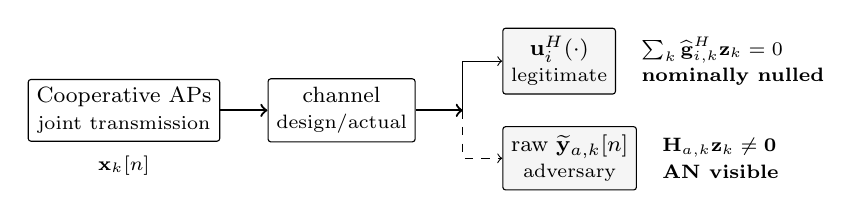
\begin{tikzpicture}[font=\footnotesize,
        block/.style={draw, rounded corners=1pt, minimum height=7mm, inner sep=3pt, align=center},
        node distance=3mm and 6mm]
        \node[block, minimum width=12mm] (TX) {Cooperative APs\\\scriptsize joint transmission};
        \node[below=0.5mm of TX, align=center] {\scriptsize $\mathbf{x}_k[n]$};
        \node[block, right=6mm of TX, minimum width=10mm] (H) {channel\\\scriptsize design/actual};
        \coordinate (br) at ($(H.east)+(6mm,0)$);
        \node[block, above right=2mm and 5mm of br, minimum width=11mm, fill=black!4] (U)
            {$\mathbf{u}_i^H(\cdot)$\\\scriptsize legitimate};
        \node[right=2mm of U, align=left] {\scriptsize $\sum_k\widehat{\mathbf{g}}_{i,k}^H\mathbf{z}_k=0$\\\scriptsize\textbf{nominally nulled}};
        \node[block, below right=2mm and 5mm of br, minimum width=11mm, fill=black!4] (R)
            {raw $\widetilde{\mathbf{y}}_{a,k}[n]$\\\scriptsize adversary};
        \node[right=2mm of R, align=left] {\scriptsize $\mathbf{H}_{a,k}\mathbf{z}_k\neq\mathbf{0}$\\\scriptsize\textbf{AN visible}};
        \draw[->, thick] (TX) -- (H);
        \draw[->, thick] (H) -- (br);
        \draw[->] (br) |- (U);
        \draw[->, dashed] (br) |- (R);
    \end{tikzpicture}
    \caption{Nominal network-wide effective-channel nulling.}
    \label{fig:asymmetry}
\end{figure}

For comparison, define the stacked AN beam $\overline{\mathbf{z}}\triangleq[\mathbf{z}_1^T,\ldots,\mathbf{z}_{N_{\mathrm{tx}}}^T]^T$ and the network-wide effective-channel matrix $\widehat{\overline{\mathbf{G}}}$, whose $i$th row is $[\widehat{\mathbf{g}}_{i,1}^H,\ldots,\widehat{\mathbf{g}}_{i,N_{\mathrm{tx}}}^H]$. Then the network-wide constraint \eqref{eq:joint-null} is equivalent to $\widehat{\overline{\mathbf{G}}}\overline{\mathbf{z}}=\mathbf{0}$. For fixed combiners, the implication $\widehat{\mathbf H}_{i,k}\mathbf z_k=\mathbf0\Rightarrow\widehat{\mathbf g}_{i,k}^H\mathbf z_k=0$ places strict physical-channel nulling inside network-wide effective-channel nulling. The rank--nullity theorem gives the corresponding dimensions
\begin{equation}
d_{\mathrm{phys}}=N_{\mathrm{tx}}[M_{\mathrm{tx}}-N_{\mathrm{UE}}M_{\mathrm{UE}}]^+,\quad
d_{\mathrm{eff}}=[N_{\mathrm{tx}}M_{\mathrm{tx}}-N_{\mathrm{UE}}]^+,
\label{eq:null-hierarchy-dim}
\end{equation}
where $[x]^+\triangleq\max(x,0)$. Network-wide effective-channel nulling imposes fewer nulling constraints than its per-AP counterpart, because it exploits cross-AP cancellation rather than requiring each AP to null its AN independently. The larger feasible shaping space leaves more freedom for geometry-consistent fake-peak shaping. 
% The latter preserves AN in the raw observations but depends on the adopted combiners and coherent AP transmission.

% The additional shaping freedom comes with increased dependence on the adopted combiners and on coherent cancellation across APs. Strict physical-channel nulling is independent of the receive combiners, but under perfect CSI it removes the AN from every per-AP raw observation and hence from the reconstruction attack. Network-wide effective-channel nulling instead preserves raw-observation AN visibility, but its null is tied to the combiners adopted in the design and requires phase coherence over the APs whose nonzero contributions cancel.

% Moreover, when $M_{\mathrm{UE}}\ge M_{\mathrm{tx}}$, each $\mathbf{H}_{a,k}$ has full column rank with probability one, so every nonzero per-AP AN component remains visible in the adversary's raw observations, whereas strict physical-channel nulling admits only $\mathbf{z}_k=\mathbf{0}$. Under the considered coherent CF-mMIMO architecture, we therefore adopt network-wide effective-channel nulling in \eqref{eq:joint-null}, which with full row rank imposes only $N_{\mathrm{UE}}$ scalar constraints and leaves $N_{\mathrm{tx}}M_{\mathrm{tx}}-N_{\mathrm{UE}}$ shaping dimensions. This choice relies on centralized beam design, a common AN stream, coherent joint transmission, and network-wide phase synchronization.

\subsection{Fake-Peak Design and Alternating Optimization}
\label{subsec:fake}
Under \eqref{eq:xk-an}, the non-self transmit component seen by the adversary becomes $\widetilde{\mathbf{x}}_k[n]=\sum_{j\neq a}\mathbf{w}_{j,k}s_j[n]+\mathbf{w}_{t,k}s_t[n]+\mathbf{z}_ks_z[n]$. Since the data, sensing, and AN symbols are mutually independent, the beampattern reconstructed in \eqref{eq:beampattern} decomposes as $\widehat{B}_k(\theta)\approx\sum_{j\neq a}|\mathbf{a}^H(\theta)\mathbf{w}_{j,k}|^2+|\mathbf{a}^H(\theta)\mathbf{w}_{t,k}|^2+|\mathbf{a}^H(\theta)\mathbf{z}_k|^2$. Within the effective-channel null space, we place the AN response along $\phi_{\mathrm{fake},k}=\angle(\mathbf{p}_{\mathrm{f}}-\mathbf{p}_k)\neq\phi_k$, where $\mathbf{p}_{\mathrm{f}}$ is a prescribed virtual location and $\phi_k=\angle(\mathbf{p}_t-\mathbf{p}_k)$ is the true direction determined by the target position $\mathbf{p}_t$. When the two directions are resolvable and the fake response dominates, the resulting AP-dependent direction lines remain consistent with $\mathbf{p}_{\mathrm{f}}$ and shift the fused estimate toward it.

Let $\Gamma_{\mathrm{comm}}$ denote the minimum required user SINR, $P_T$ the per-AP transmit-power budget, and $\rho$ the ratio between the fake-direction AN response and the useful-beam power in the true direction. Collect the transmit variables as $\mathcal{W}\triangleq\{\mathbf{W}_k\}_{k=1}^{N_{\mathrm{tx}}}$ and $\mathcal{Z}\triangleq\{\mathbf{z}_k\}_{k=1}^{N_{\mathrm{tx}}}$. Since the central processor designs the beams from the estimated CSI, define $h_i(\mathcal W)\triangleq\sum_k\widehat{\mathbf g}_{i,k}^H\mathbf w_{i,k}$ and
\begin{equation}
\widehat{\gamma}_i=\frac{|h_i(\mathcal W)|^2}{\mathcal{I}_i(\mathcal{W},\mathcal{Z})},
\label{eq:sinr-nominal}
\end{equation}
where $\mathcal{I}_i(\mathcal{W},\mathcal{Z})={\textstyle\sum_{j\neq i}}\big|{\textstyle\sum_k}\widehat{\mathbf{g}}_{i,k}^H\mathbf{w}_{j,k}\big|^2+\big|{\textstyle\sum_k}\widehat{\mathbf{g}}_{i,k}^H\mathbf{w}_{t,k}\big|^2+\big|{\textstyle\sum_k}\widehat{\mathbf{g}}_{i,k}^H\mathbf{z}_k\big|^2+\sigma_i^2$. On this basis, the secure beam design can be formulated as
\begin{subequations}
\begin{align}
\max_{\{\mathbf{W}_k,\mathbf{z}_k,\mathbf{u}_i\}} \quad & \sum_{k=1}^{N_{\mathrm{tx}}}c_k\left\|\mathbf{a}^H(\phi_k)\mathbf{W}_k\right\|_F^2 \label{prob:obj}\\
\text{s.t.}\quad & \widehat{\gamma}_i\ge \Gamma_{\mathrm{comm}},\;\forall i, \label{prob:sinr}\\
& \|\mathbf{u}_i\|=1,\;\forall i, \label{prob:unit-norm}\\
& \textstyle\sum_{j=1}^{N_{\mathrm{UE}}}\|\mathbf{w}_{j,k}\|^2+\|\mathbf{w}_{t,k}\|^2+\|\mathbf{z}_k\|^2\le P_T,\;\forall k, \label{prob:power}\\
& \textstyle\sum_{k=1}^{N_{\mathrm{tx}}}\widehat{\mathbf{g}}_{i,k}^H\mathbf{z}_k=0,\;\forall i, \label{prob:null}\\
& \textstyle\sum_{k=1}^{N_{\mathrm{tx}}}\widehat{\mathbf{g}}_{i,k}^H\mathbf{w}_{t,k}=0,\;\forall i, \label{prob:null-t}\\
& \left|\mathbf{a}^H(\phi_{\mathrm{fake},k})\mathbf{z}_k\right|^2 \ge \rho\left\|\mathbf{a}^H(\phi_k)\mathbf{W}_k\right\|_F^2,\;\forall k. \label{prob:fake}
\end{align}
\end{subequations}
Constraint \eqref{prob:sinr} enforces communication QoS, \eqref{prob:power} limits the per-AP power, and \eqref{prob:null}--\eqref{prob:null-t} place the stacked AN and sensing beams in $\mathcal{N}(\widehat{\overline{\mathbf{G}}})$, thereby removing both terms at the prescribed legitimate combiners. Although the adversary subtracts its own stream, \eqref{prob:fake} retains the full $\mathbf W_k$, because the adversary is indistinguishable from an ordinary user and the central processor therefore cannot identify $a$. The constraint is thus enforced conservatively for every candidate adversary. With $\mathbf W_{-a,k}$ denoting $\mathbf W_k$ without $\mathbf w_{a,k}$, define $S_k=\|\mathbf a^H(\phi_k)\mathbf W_{-a,k}\|_F^2$, $F_k=|\mathbf a^H(\phi_{\mathrm{fake},k})\mathbf z_k|^2$, and $T_k=|\mathbf a^H(\phi_k)\mathbf z_k|^2$. Then \eqref{prob:fake} gives $S_k\le F_k/\rho$. If $T_k/F_k\le1/M_{\mathrm{tx}}$, the ideal covariance decomposition yields
\begin{equation}
\widehat B_k(\phi_{\mathrm{fake},k})-\widehat B_k(\phi_k)
\ge F_k-S_k-T_k
\ge F_k\left(1-\frac{1}{\rho}-\frac{1}{M_{\mathrm{tx}}}\right).
\label{eq:fake-dominance}
\end{equation}
Hence, $\rho>M_{\mathrm{tx}}/(M_{\mathrm{tx}}-1)$ is sufficient for the fake-direction response to exceed the true-direction response. The prescribed $\mathbf p_{\mathrm f}$ must therefore yield resolvable true and fake directions. Since $s_z[n]$ is known at the sensing receivers and independent of $s_t[n]$, ideal matched filtering separates their echoes.

For fixed combiners, the transmit subproblem is nonconvex. Define $\mathbf{A}_k=\mathbf{a}(\phi_k)\mathbf{a}^H(\phi_k)$, $\mathbf{A}_{\mathrm{f},k}=\mathbf{a}(\phi_{\mathrm{fake},k})\mathbf{a}^H(\phi_{\mathrm{fake},k})$, and, for $\mathbf A\succeq\mathbf0$,
\begin{equation}
\mathcal{L}_{\mathbf A}(\mathbf X;\mathbf X_0)
\triangleq2\Re\!\left\{\mathrm{Tr}[(\mathbf A\mathbf X_0)^H\mathbf X]\right\}
-\mathrm{Tr}(\mathbf X_0^H\mathbf A\mathbf X_0),
\label{eq:affine-lb}
\end{equation}
which lower-bounds $\mathrm{Tr}(\mathbf X^H\mathbf A\mathbf X)$ at $\mathbf X_0$. At CCCP iteration $v$, every convex quadratic that is maximized or subtracted is replaced by its affine lower bound at the current iterate. For the sensing objective this gives the surrogate $\widetilde f_0^{(v)}(\mathcal W)={\textstyle\sum_k}c_k\mathcal{L}_{\mathbf A_k}(\mathbf W_k;\mathbf W_k^{(v)})$, and for the fake-direction response it gives $\widetilde\zeta_k=\mathcal{L}_{\mathbf A_{\mathrm{f},k}}(\mathbf z_k;\mathbf z_k^{(v)})$. Since $h_i$ is a scalar aggregating all APs rather than a per-AP quadratic form, \eqref{eq:affine-lb} does not apply directly, and the affine lower bound of $|h_i(\mathcal W)|^2$ is written out as $\widetilde h_i=2\Re\{h_i^*(\mathcal W^{(v)})h_i(\mathcal W)\}-|h_i(\mathcal W^{(v)})|^2$.
The CCCP transmit update \cite{scutari2017sca} is
\begin{subequations}\label{eq:tx-cvx}
\begin{align}
\max_{\{\mathbf{W}_k,\mathbf{z}_k\}}\quad & \widetilde f_0^{(v)}(\mathcal{W})\\
\text{s.t.}\quad & \Gamma_{\mathrm{comm}}\mathcal{I}_i(\mathcal{W},\mathcal{Z})-\widetilde h_i\le 0,\ \forall i,\\
& \eqref{prob:power},\ \eqref{prob:null},\ \eqref{prob:null-t},\\
& \rho\,\mathrm{Tr}(\mathbf{W}_k^H\mathbf{A}_k\mathbf{W}_k)-\widetilde\zeta_k\le 0,\ \forall k.
\end{align}
\end{subequations}
This is a convex quadratically constrained problem because its objective is affine and all negative convex terms have been replaced by their affine lower bounds. For fixed combiners, tightness preserves feasibility of the current point. Thus, letting $f_0(\mathcal W)\triangleq\sum_k c_k\mathrm{Tr}(\mathbf W_k^H\mathbf A_k\mathbf W_k)$ and assuming that the surrogate problem is solved exactly, we obtain
\begin{equation}
f_0(\mathcal W^{(v+1)})
\ge \widetilde f_0^{(v)}(\mathcal W^{(v+1)})
\ge \widetilde f_0^{(v)}(\mathcal W^{(v)})
=f_0(\mathcal W^{(v)}),
\label{eq:cccp-monotonicity}
\end{equation}
where the two inequalities and the equality follow from global minorization, subproblem optimality, and tangency, respectively. Hence, each feasible fixed-combiner CCCP update is non-decreasing in the original objective.

For fixed transmit beams, let $\mathbf{q}_{i,j}=\sum_k\widehat{\mathbf{H}}_{i,k}\mathbf{w}_{j,k}$, $\mathbf{q}_{i,t}=\sum_k\widehat{\mathbf{H}}_{i,k}\mathbf{w}_{t,k}$, $\mathbf{q}_{i,z}=\sum_k\widehat{\mathbf{H}}_{i,k}\mathbf{z}_k$, $\mathbf{Q}_i=[\mathbf{q}_{i,z},\mathbf{q}_{i,t}]$, and
\begin{equation}
\mathbf{R}_i=\sum_{j\neq i}\mathbf{q}_{i,j}\mathbf{q}_{i,j}^H+\mathbf{q}_{i,t}\mathbf{q}_{i,t}^H+\mathbf{q}_{i,z}\mathbf{q}_{i,z}^H+\sigma_i^2\mathbf{I}_{M_{\mathrm{UE}}}.
\label{eq:interference-cov}
\end{equation}
Since $\mathbf R_i\succ\mathbf0$, maximizing $|\mathbf{u}_i^H\mathbf{q}_{i,i}|^2/(\mathbf{u}_i^H\mathbf{R}_i\mathbf{u}_i)$ subject to $\mathbf{Q}_i^H\mathbf{u}_i=\mathbf0$ and $\|\mathbf u_i\|=1$ gives the MMSE update
\begin{equation}
\widetilde{\mathbf{u}}_i
=\mathbf{R}_i^{-1}\mathbf{q}_{i,i}
-\mathbf{R}_i^{-1}\mathbf{Q}_i
\left(\mathbf{Q}_i^H\mathbf{R}_i^{-1}\mathbf{Q}_i\right)^\dagger
\mathbf{Q}_i^H\mathbf{R}_i^{-1}\mathbf{q}_{i,i},
\label{eq:mmse}
\end{equation}
where $\mathbf{u}_i={\widetilde{\mathbf{u}}_i}/{\|\widetilde{\mathbf{u}}_i\|}$. To verify the optimality, let $\boldsymbol{\alpha}_i=(\mathbf Q_i^H\mathbf R_i^{-1}\mathbf Q_i)^\dagger\mathbf Q_i^H\mathbf R_i^{-1}\mathbf q_{i,i}$. Then we have $\mathbf Q_i^H\widetilde{\mathbf u}_i=\mathbf0$ and $\mathbf R_i\widetilde{\mathbf u}_i=\mathbf q_{i,i}-\mathbf Q_i\boldsymbol{\alpha}_i$. Thus, for any feasible $\mathbf u_i$, Cauchy--Schwarz in the $\mathbf R_i$-inner product gives
\begin{equation}
\frac{|\mathbf u_i^H\mathbf q_{i,i}|^2}{\mathbf u_i^H\mathbf R_i\mathbf u_i}
=\frac{|\mathbf u_i^H\mathbf R_i\widetilde{\mathbf u}_i|^2}{\mathbf u_i^H\mathbf R_i\mathbf u_i}
\le \widetilde{\mathbf u}_i^H\mathbf R_i\widetilde{\mathbf u}_i,
\label{eq:mmse-optimality}
\end{equation}
with equality when $\mathbf u_i$ is proportional to $\widetilde{\mathbf u}_i$. Therefore, the vector in \eqref{eq:mmse} is globally optimal whenever $\widetilde{\mathbf u}_i\neq\mathbf0$ and the constraint null space is nonempty.

The transmit beams are initialized along the dominant user-channel, true, and fake steering directions. If the first update \eqref{eq:tx-cvx} is solvable, its global lower bounds ensure original feasibility, which the constrained-MMSE step preserves by keeping the preceding combiner feasible. Each exact transmit update is non-decreasing in $f_0$ by \eqref{eq:cccp-monotonicity}, the MMSE step leaves $f_0$ unchanged, and per-AP power constraints bound $f_0$ above, so its values converge. Iterations stop once the relative change in $f_0$ falls below $\varepsilon_{\mathrm{tol}}$, and convergence of the variables or to a joint KKT point is not claimed.

\subsection{Imperfect-CSI Extension}
\label{subsec:robust-formulation}
Channel-estimation errors could destroy the nominal null. Write $\mathbf{H}_{i,k}=\widehat{\mathbf{H}}_{i,k}+\mathbf{E}_{i,k}$ and let $\widehat{\mathcal H}$ collect all channel estimates. Under the LMMSE model, $\mathbf E_{i,k}$ is independent of $\widehat{\mathcal H}$ and across links, with i.i.d. $\mathcal{CN}(0,\widetilde\beta_{i,k})$ entries, where $\widetilde\beta_{i,k}=\epsilon_{i,k}^{2}\beta_{i,k}$ and $\epsilon_{i,k}^{2}=\sigma_{\mathrm{p}}^{2}/(\tau_{\mathrm{p}}p_i^{\mathrm{p}}\beta_{i,k}+\sigma_{\mathrm{p}}^{2})$. If the unit-norm combiner $\mathbf u_i$ and beams $\{\mathbf v_k\}$ depend only on $\widehat{\mathcal H}$, then
\begin{equation}
\begin{aligned}
&\mathbb{E}\!\left\{\left.\Big|{\textstyle\sum_k}\mathbf{u}_i^{H}\mathbf{H}_{i,k}\mathbf{v}_k\Big|^{2}\,\right|\widehat{\mathcal{H}}\right\}\\
&\qquad=\Big|{\textstyle\sum\nolimits_k}\mathbf{u}_i^{H}\widehat{\mathbf{H}}_{i,k}\mathbf{v}_k\Big|^{2}
+\sum\nolimits_{k=1}^{N_{\mathrm{tx}}}\widetilde{\beta}_{i,k}\|\mathbf{v}_k\|^{2},
\end{aligned}
\label{eq:beamsplit}
\end{equation}
because the conditional error term is zero mean with variance $\sum_k\widetilde\beta_{i,k}\|\mathbf v_k\|^2$, so its cross term with the estimated-channel component vanishes. Setting $\mathbf v_k=\mathbf z_k$ and applying \eqref{prob:null} gives
\begin{equation}
\mathbb{E}\!\left\{\left.\Big|{\textstyle\sum_k}\mathbf{u}_i^{H}\mathbf{H}_{i,k}\mathbf{z}_k\Big|^{2}\,\right|\widehat{\mathcal{H}}\right\}
=\sum\nolimits_{k=1}^{N_{\mathrm{tx}}}\widetilde{\beta}_{i,k}\|\mathbf{z}_k\|^{2}.
\label{eq:leakpower}
\end{equation}
Thus, for fixed per-AP AN powers, the residual is independent of the AN direction under the isotropic error model. Summing \eqref{eq:beamsplit} over all data, sensing, and AN beams gives the CSI-error interference floor
\begin{equation}
L_i^{\mathrm{csi}}=\sum_{k=1}^{N_{\mathrm{tx}}}\widetilde{\beta}_{i,k}\,P_k,
\quad
P_k\triangleq\sum_{j=1}^{N_{\mathrm{UE}}}\|\mathbf{w}_{j,k}\|^{2}
+\|\mathbf{w}_{t,k}\|^{2}+\|\mathbf{z}_k\|^{2},
\label{eq:csi-floor}
\end{equation}
which includes the useful-beam estimation error and depends on each AP's total radiated power.

% The effective-channel null additionally assumes that each user applies the combiner adopted by the central processor and that the APs maintain relative phase coherence. Combiner disagreement and differential AP phase offsets are implementation impairments outside the present CSI-uncertainty model and are assumed to be controlled through receiver-side combiner coordination and network synchronization \cite{ozdogan2019phaseshift}.

Since $L_i^{\mathrm{csi}}$ is a convex quadratic form, define the updated interference-plus-noise $\overline{\mathcal{I}}_i(\mathcal{W},\mathcal{Z})=\mathcal{I}_i(\mathcal{W},\mathcal{Z})+L_i^{\mathrm{csi}}$ and the corresponding robust SINR $\overline{\gamma}_i={|h_i(\mathcal{W})|^{2}}/{\overline{\mathcal{I}}_i(\mathcal{W},\mathcal{Z})}$. The resulting robust formulation of \eqref{prob:obj}--\eqref{prob:fake} is
\begin{subequations}\label{prob:robust}
\begin{align}
\max_{\{\mathbf{W}_k,\mathbf{z}_k,\mathbf{u}_i\}}\quad
& \sum_{k=1}^{N_{\mathrm{tx}}}c_k\left\|\mathbf{a}^{H}(\phi_k)\mathbf{W}_k\right\|_F^{2}\\
\text{s.t.}\quad & \overline{\gamma}_i\ge\Gamma_{\mathrm{comm}},\;\forall i,
\label{prob:robust-sinr}\\
& \eqref{prob:unit-norm},\;\eqref{prob:power},\;\eqref{prob:null},\;\eqref{prob:null-t},\;\eqref{prob:fake}.
\end{align}
\end{subequations}
The same CCCP--MMSE updates apply by replacing $\mathcal I_i$ with $\overline{\mathcal I}_i$ in \eqref{eq:tx-cvx} and $\sigma_i^2\mathbf I_{M_{\mathrm{UE}}}$ with $(\sigma_i^2+L_i^{\mathrm{csi}})\mathbf I_{M_{\mathrm{UE}}}$ in \eqref{eq:interference-cov}. The added positive quadratic term preserves convexity of the transmit update. Moreover, $\overline{\gamma}_i\le\widehat{\gamma}_i$, so the robust feasible set is contained in the nominal one and the two coincide as $\epsilon_{i,k}^2\to0$. Under the same feasibility and exact-solve assumptions, the preceding objective-value convergence argument remains valid. This error-averaged formulation controls conditional mean interference under the adopted isotropic LMMSE model. 

% It does not impose a per-realization or worst-case SINR guarantee, so its outage behavior on the actual channels is evaluated in Fig.~\ref{fig:outage-nmse}.

% The error-averaged robustness term leaves the algorithmic structure and the convex form of the transmit update unchanged, at the cost of one additional quadratic term per iteration. The tightened SINR constraint withdraws power from the sensing and AN beams, so the robust design trades some sensing and privacy performance for its outage guarantee, a tradeoff Section~\ref{subsec:robust-results} quantifies.

\section{Simulation Results}
\label{sec:sim}
% This section evaluates the proposed design in five stages. We first specify the simulation setup, baselines, and leakage metrics. We then examine the numerical stabilization of the algorithm and the fake-peak mechanism of Section~\ref{sec:design}, together with the effective-channel nulling mechanism of Section~\ref{sec:nulling}. We next validate the CSI-error-induced interference analysis of Section~\ref{subsec:leakage}, evaluate the end-to-end localization deception and privacy--sensing--power tradeoff, and finally assess the robust design under imperfect CSI.

\subsection{Simulation Setup and Metrics}
\label{subsec:sim-setup}

Table~\ref{tab:sim-params} lists the default parameters. Throughout, the beams are designed from LMMSE channel estimates, whereas the adversary's reconstruction and the realized SINRs are evaluated on the actual channels. The realized AN-power ratio is $\eta=\sum_k\|\mathbf{z}_k\|^2/\sum_k\!\left(\sum_i\|\mathbf{w}_{i,k}\|^2+\|\mathbf{w}_{t,k}\|^2+\|\mathbf{z}_k\|^2\right)$.

\begin{table}[t]
\centering
\caption{Default Simulation Parameters}
\label{tab:sim-params}
\small
\begin{tabular}{@{}p{0.47\columnwidth}p{0.46\columnwidth}@{}}
\hline
Parameter & Value\\
\hline
Network size $(N_{\mathrm{tx}},N_{\mathrm{rx}},N_{\mathrm{UE}})$ & $(8,4,4)$\\
Antenna counts $(M_{\mathrm{tx}},M_{\mathrm{UE}})$ & $(16,16)$\\
Carrier frequency & $1.9$~GHz\\
Power/SINR $(P_T,\Gamma_{\mathrm{comm}})$ & $(30~\mathrm{dBm},10~\mathrm{dB})$\\
Noise powers $(\sigma_i^2,\sigma_{\mathrm{rx}}^2,\sigma_{\mathrm{p}}^2)$ & $(-94,-94,-94)$~dBm\\
Transmit/receive AP coordinates & \begin{tabular}[t]{@{}l@{}}Tx: $(\pm200,\pm200),(0,\pm200)$\\\phantom{Tx: }$(\pm200,0)$~m; Rx:\\\phantom{Tx: }$(\pm150,\pm150)$~m\end{tabular}\\
True/fake coordinates & \begin{tabular}[t]{@{}l@{}}$(-75,75)/(5,-25)$~m\end{tabular}\\
Pilot length/total power $(\tau_{\mathrm{p}},P_{\mathrm{p}})$ & $(64,20~\mathrm{dBm})$\\
Snapshots/grid cell $(N,\Delta_{\mathrm{g}})$ & $(128,10~\mathrm{m}\times10~\mathrm{m})$\\
\hline
\end{tabular}
\end{table}

Five candidate designs are included for comparison. The \emph{no-AN} baseline maximizes the sensing objective under the QoS and power constraints. The \emph{null-space-only AN} baseline projects Gaussian AN onto \(\mathcal N(\widehat{\overline{\mathbf G}})\) without fake-peak shaping, whereas the \emph{MI-minimizing AN} baseline adapts \cite{zou2024securing} to minimize true-direction leakage within the same null space. The proposed nominal and robust designs solve \eqref{prob:obj}--\eqref{prob:fake} and \eqref{prob:robust}, respectively. Localization succeeds when the fused estimate lies in the target's grid cell of size $\Delta_{\mathrm{g}}$, while localization error is its Euclidean distance from the target.

\subsection{Results Discussion}
\label{subsec:localization-results}

\begin{figure}[!t]
    \centering
    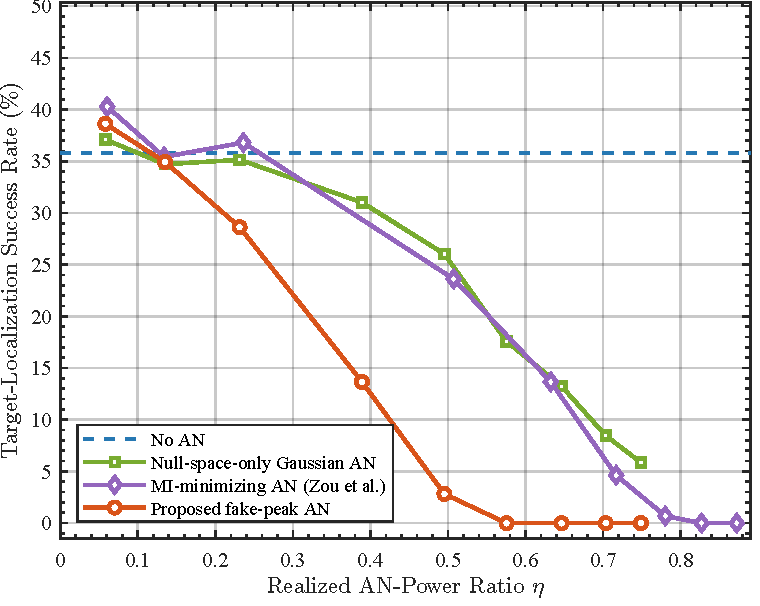
\includegraphics[width=0.8\columnwidth]{localization_success_tvt.pdf}
    \caption{Target-localization success rate versus the realized AN-power ratio $\eta$.}
    \label{fig:localization-success}
\end{figure}

For $M_{\mathrm{tx}}=16$, \eqref{eq:fake-dominance} gives the sufficient condition $\rho>1.07$. Sweeping $\rho$ over $[0.05,3.5]$ traces the realized AN-power ratio $\eta$ reported on the horizontal axis. Fig.~\ref{fig:localization-success} reports the target-localization success rate versus $\eta$, at the estimation quality implied by the tabulated pilot configuration. Without AN the adversary succeeds in $35.8\%$ of the channel realizations. At $\eta\approx0.50$, the null-space-only and MI-minimizing baselines still give $26.0\%$ and $23.6\%$, whereas the proposed design drops to $2.8\%$ and reaches $0\%$ at $\eta\approx0.58$. The MI-minimizing design requires $\eta\approx0.78$ to approach a comparable level. The key difference is geometry-consistent shaping. Unstructured or leakage-minimizing AN perturbs individual beampatterns but does not force the residual peaks to intersect at one false position, whereas the proposed constraints couple fake directions through the common virtual location, drawing multi-AP fusion toward a coherent alternative.

\begin{figure}[!t]
    \centering
    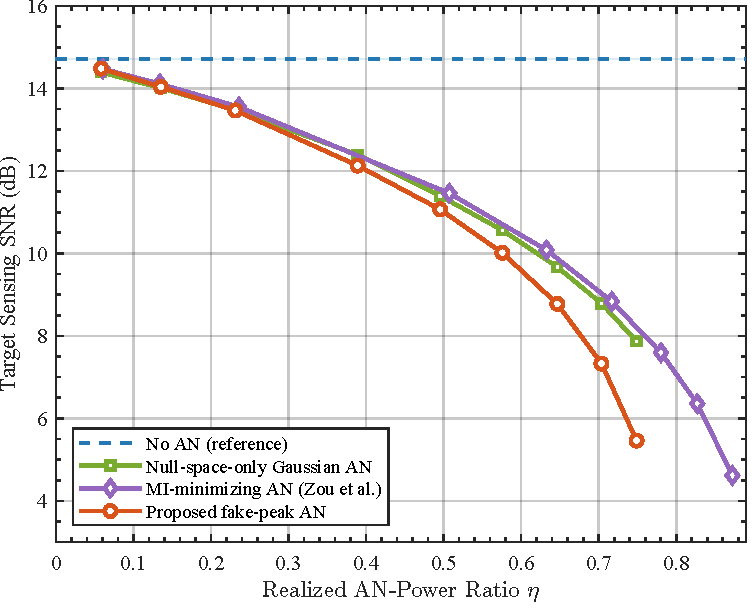
\includegraphics[width=0.8\columnwidth]{sensing_snr_final.pdf}
    \caption{Target sensing SNR versus the realized AN-power ratio $\eta$ at the same paired operating points.}
    \label{fig:sensing-snr}
\end{figure}

Fig.~\ref{fig:sensing-snr} reports the sensing cost at the same paired operating points. The no-AN reference is $14.7$~dB. At $\eta\approx0.50$, the proposed, null-space-only, and MI-minimizing designs yield $11.1$, $11.4$, and $11.5$~dB, a $3.6$~dB loss for the proposed design relative to the no-AN reference and only $0.3$--$0.4$~dB additional loss relative to the baselines while achieving a much lower localization success rate. At larger $\eta$ the proposed curve decreases faster due to the more restrictive fake-peak shaping constraint. Jointly, at $\eta\approx0.50$ all three schemes sacrifice similar sensing SNR, yet only the proposed design reduces localization success to $2.8\%$, identifying this as a favorable operating region.

% The operator can therefore select the operating point according to the required privacy level without a fixed performance penalty.

Fig.~\ref{fig:outage-nmse} evaluates QoS on the actual channels, now sweeping a common link NMSE directly rather than fixing it through the pilot configuration, so as to isolate the effect of CSI accuracy. At $-10$~dB NMSE, the no-AN baseline already incurs $75.1\%$ outage, whereas the robust design reduces outage from $18.6\%$ (nominal) to $1.6\%$ at a cost of $0.19$~dB in sensing SNR relative to the nominal design. The high outage of the no-AN baseline arises because it attains a higher sensing SNR by operating with a smaller communication-SINR margin, making it more vulnerable to channel uncertainty. The advantage widens at larger NMSE, where at $-4$~dB the robust design still holds outage to $31.6\%$ while the other three variants all exceed $99\%$. 

% The null-space-only AN gives a closely matched $18.3\%$ outage, indicating that fake-peak shaping introduces only a small additional outage penalty in this setting and that CSI mismatch is the dominant source of the residual outage.

\begin{figure}[!t]
    \centering
    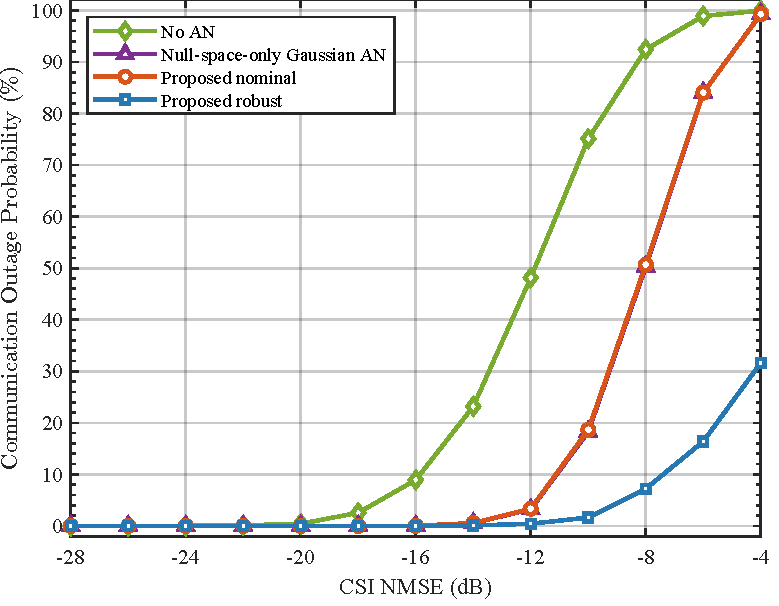
\includegraphics[width=0.8\columnwidth]{outage_vs_nmse.pdf}
    \caption{Communication outage probability $\Pr\{\min_i\gamma_i^{\mathrm{AN}}<\Gamma_{\mathrm{comm}}\}$ on the actual channel versus the CSI NMSE for four design variants.}
    \label{fig:outage-nmse}
\end{figure}

\section{Conclusion}
\label{sec:conclusion}
This correspondence proposed a fake-peak AN design for CF-mMIMO ISAC that exploits the receive-processing asymmetry between post-combining detection and raw-sample reconstruction. Network-wide effective-channel nulling preserves the AN in the adversary's observations, and geometry-consistent shaping displaces the reconstructed dominant peaks away from the target. At $\eta\approx0.50$, the design lowers localization success from $35.8\%$ to $2.8\%$ with a $3.6$~dB sensing-SNR loss and a $20$-percentage-point margin over the MI-minimizing baseline.

\bibliographystyle{IEEEtran}
\bibliography{references}

\end{document}
